% Options for packages loaded elsewhere
\PassOptionsToPackage{unicode}{hyperref}
\PassOptionsToPackage{hyphens}{url}
%
\documentclass[
]{article}
\usepackage{amsmath,amssymb}
\usepackage{iftex}
\ifPDFTeX
  \usepackage[T1]{fontenc}
  \usepackage[utf8]{inputenc}
  \usepackage{textcomp} % provide euro and other symbols
\else % if luatex or xetex
  \usepackage{unicode-math} % this also loads fontspec
  \defaultfontfeatures{Scale=MatchLowercase}
  \defaultfontfeatures[\rmfamily]{Ligatures=TeX,Scale=1}
\fi
\usepackage{lmodern}
\ifPDFTeX\else
  % xetex/luatex font selection
\fi
% Use upquote if available, for straight quotes in verbatim environments
\IfFileExists{upquote.sty}{\usepackage{upquote}}{}
\IfFileExists{microtype.sty}{% use microtype if available
  \usepackage[]{microtype}
  \UseMicrotypeSet[protrusion]{basicmath} % disable protrusion for tt fonts
}{}
\makeatletter
\@ifundefined{KOMAClassName}{% if non-KOMA class
  \IfFileExists{parskip.sty}{%
    \usepackage{parskip}
  }{% else
    \setlength{\parindent}{0pt}
    \setlength{\parskip}{6pt plus 2pt minus 1pt}}
}{% if KOMA class
  \KOMAoptions{parskip=half}}
\makeatother
\usepackage{xcolor}
\usepackage[margin=1in]{geometry}
\usepackage{color}
\usepackage{fancyvrb}
\newcommand{\VerbBar}{|}
\newcommand{\VERB}{\Verb[commandchars=\\\{\}]}
\DefineVerbatimEnvironment{Highlighting}{Verbatim}{commandchars=\\\{\}}
% Add ',fontsize=\small' for more characters per line
\usepackage{framed}
\definecolor{shadecolor}{RGB}{248,248,248}
\newenvironment{Shaded}{\begin{snugshade}}{\end{snugshade}}
\newcommand{\AlertTok}[1]{\textcolor[rgb]{0.94,0.16,0.16}{#1}}
\newcommand{\AnnotationTok}[1]{\textcolor[rgb]{0.56,0.35,0.01}{\textbf{\textit{#1}}}}
\newcommand{\AttributeTok}[1]{\textcolor[rgb]{0.13,0.29,0.53}{#1}}
\newcommand{\BaseNTok}[1]{\textcolor[rgb]{0.00,0.00,0.81}{#1}}
\newcommand{\BuiltInTok}[1]{#1}
\newcommand{\CharTok}[1]{\textcolor[rgb]{0.31,0.60,0.02}{#1}}
\newcommand{\CommentTok}[1]{\textcolor[rgb]{0.56,0.35,0.01}{\textit{#1}}}
\newcommand{\CommentVarTok}[1]{\textcolor[rgb]{0.56,0.35,0.01}{\textbf{\textit{#1}}}}
\newcommand{\ConstantTok}[1]{\textcolor[rgb]{0.56,0.35,0.01}{#1}}
\newcommand{\ControlFlowTok}[1]{\textcolor[rgb]{0.13,0.29,0.53}{\textbf{#1}}}
\newcommand{\DataTypeTok}[1]{\textcolor[rgb]{0.13,0.29,0.53}{#1}}
\newcommand{\DecValTok}[1]{\textcolor[rgb]{0.00,0.00,0.81}{#1}}
\newcommand{\DocumentationTok}[1]{\textcolor[rgb]{0.56,0.35,0.01}{\textbf{\textit{#1}}}}
\newcommand{\ErrorTok}[1]{\textcolor[rgb]{0.64,0.00,0.00}{\textbf{#1}}}
\newcommand{\ExtensionTok}[1]{#1}
\newcommand{\FloatTok}[1]{\textcolor[rgb]{0.00,0.00,0.81}{#1}}
\newcommand{\FunctionTok}[1]{\textcolor[rgb]{0.13,0.29,0.53}{\textbf{#1}}}
\newcommand{\ImportTok}[1]{#1}
\newcommand{\InformationTok}[1]{\textcolor[rgb]{0.56,0.35,0.01}{\textbf{\textit{#1}}}}
\newcommand{\KeywordTok}[1]{\textcolor[rgb]{0.13,0.29,0.53}{\textbf{#1}}}
\newcommand{\NormalTok}[1]{#1}
\newcommand{\OperatorTok}[1]{\textcolor[rgb]{0.81,0.36,0.00}{\textbf{#1}}}
\newcommand{\OtherTok}[1]{\textcolor[rgb]{0.56,0.35,0.01}{#1}}
\newcommand{\PreprocessorTok}[1]{\textcolor[rgb]{0.56,0.35,0.01}{\textit{#1}}}
\newcommand{\RegionMarkerTok}[1]{#1}
\newcommand{\SpecialCharTok}[1]{\textcolor[rgb]{0.81,0.36,0.00}{\textbf{#1}}}
\newcommand{\SpecialStringTok}[1]{\textcolor[rgb]{0.31,0.60,0.02}{#1}}
\newcommand{\StringTok}[1]{\textcolor[rgb]{0.31,0.60,0.02}{#1}}
\newcommand{\VariableTok}[1]{\textcolor[rgb]{0.00,0.00,0.00}{#1}}
\newcommand{\VerbatimStringTok}[1]{\textcolor[rgb]{0.31,0.60,0.02}{#1}}
\newcommand{\WarningTok}[1]{\textcolor[rgb]{0.56,0.35,0.01}{\textbf{\textit{#1}}}}
\usepackage{graphicx}
\makeatletter
\def\maxwidth{\ifdim\Gin@nat@width>\linewidth\linewidth\else\Gin@nat@width\fi}
\def\maxheight{\ifdim\Gin@nat@height>\textheight\textheight\else\Gin@nat@height\fi}
\makeatother
% Scale images if necessary, so that they will not overflow the page
% margins by default, and it is still possible to overwrite the defaults
% using explicit options in \includegraphics[width, height, ...]{}
\setkeys{Gin}{width=\maxwidth,height=\maxheight,keepaspectratio}
% Set default figure placement to htbp
\makeatletter
\def\fps@figure{htbp}
\makeatother
\setlength{\emergencystretch}{3em} % prevent overfull lines
\providecommand{\tightlist}{%
  \setlength{\itemsep}{0pt}\setlength{\parskip}{0pt}}
\setcounter{secnumdepth}{-\maxdimen} % remove section numbering
\usepackage{booktabs}
\usepackage{longtable}
\usepackage{array}
\usepackage{multirow}
\usepackage{wrapfig}
\usepackage{float}
\usepackage{colortbl}
\usepackage{pdflscape}
\usepackage{tabu}
\usepackage{threeparttable}
\usepackage{threeparttablex}
\usepackage[normalem]{ulem}
\usepackage{makecell}
\usepackage{xcolor}
\ifLuaTeX
  \usepackage{selnolig}  % disable illegal ligatures
\fi
\usepackage{bookmark}
\IfFileExists{xurl.sty}{\usepackage{xurl}}{} % add URL line breaks if available
\urlstyle{same}
\hypersetup{
  pdftitle={Dados Videos},
  pdfauthor={Vinnicius Pereira},
  hidelinks,
  pdfcreator={LaTeX via pandoc}}

\title{Dados Videos}
\author{Vinnicius Pereira}
\date{2025-04-12}

\begin{document}
\maketitle

\begin{Shaded}
\begin{Highlighting}[]
\FunctionTok{library}\NormalTok{(readxl)}
\FunctionTok{library}\NormalTok{(ggplot2)}
\FunctionTok{library}\NormalTok{(summarytools)}
\FunctionTok{library}\NormalTok{(GGally)}
\end{Highlighting}
\end{Shaded}

\begin{verbatim}
## Registered S3 method overwritten by 'GGally':
##   method from   
##   +.gg   ggplot2
\end{verbatim}

\begin{Shaded}
\begin{Highlighting}[]
\FunctionTok{library}\NormalTok{(ggpubr)}
\FunctionTok{library}\NormalTok{(mice)}
\end{Highlighting}
\end{Shaded}

\begin{verbatim}
## 
## Anexando pacote: 'mice'
\end{verbatim}

\begin{verbatim}
## O seguinte objeto é mascarado por 'package:stats':
## 
##     filter
\end{verbatim}

\begin{verbatim}
## Os seguintes objetos são mascarados por 'package:base':
## 
##     cbind, rbind
\end{verbatim}

\begin{Shaded}
\begin{Highlighting}[]
\FunctionTok{library}\NormalTok{(shiny)}
\FunctionTok{library}\NormalTok{(colourpicker)}
\end{Highlighting}
\end{Shaded}

\begin{verbatim}
## 
## Anexando pacote: 'colourpicker'
\end{verbatim}

\begin{verbatim}
## O seguinte objeto é mascarado por 'package:shiny':
## 
##     runExample
\end{verbatim}

\begin{Shaded}
\begin{Highlighting}[]
\FunctionTok{library}\NormalTok{(flexdashboard)}
\FunctionTok{library}\NormalTok{(tidyverse)}
\end{Highlighting}
\end{Shaded}

\begin{verbatim}
## -- Attaching core tidyverse packages ------------------------ tidyverse 2.0.0 --
## v dplyr     1.1.4     v readr     2.1.5
## v forcats   1.0.0     v stringr   1.5.1
## v lubridate 1.9.4     v tibble    3.2.1
## v purrr     1.0.4     v tidyr     1.3.1
\end{verbatim}

\begin{verbatim}
## -- Conflicts ------------------------------------------ tidyverse_conflicts() --
## x dplyr::filter() masks mice::filter(), stats::filter()
## x dplyr::lag()    masks stats::lag()
## x tibble::view()  masks summarytools::view()
## i Use the conflicted package (<http://conflicted.r-lib.org/>) to force all conflicts to become errors
\end{verbatim}

\begin{Shaded}
\begin{Highlighting}[]
\FunctionTok{library}\NormalTok{(knitr)}
\FunctionTok{library}\NormalTok{(rmarkdown)}
\FunctionTok{library}\NormalTok{(kableExtra)}
\end{Highlighting}
\end{Shaded}

\begin{verbatim}
## 
## Anexando pacote: 'kableExtra'
## 
## O seguinte objeto é mascarado por 'package:dplyr':
## 
##     group_rows
\end{verbatim}

\begin{Shaded}
\begin{Highlighting}[]
\FunctionTok{library}\NormalTok{(stargazer)}
\end{Highlighting}
\end{Shaded}

\begin{verbatim}
## 
## Please cite as: 
## 
##  Hlavac, Marek (2022). stargazer: Well-Formatted Regression and Summary Statistics Tables.
##  R package version 5.2.3. https://CRAN.R-project.org/package=stargazer
\end{verbatim}

\begin{Shaded}
\begin{Highlighting}[]
\FunctionTok{library}\NormalTok{(shiny)}
\FunctionTok{library}\NormalTok{(mice)}
\end{Highlighting}
\end{Shaded}

\subsection{Introdução}\label{introduuxe7uxe3o}

A base de dados utilizada neste projeto se chama
\texttt{dados\_videos.xlsx} e contém informações sobre vídeos curtos e
suas métricas de engajamento. A escolha se deu por apresentar variáveis
numéricas suficientes para a análise e por conter dados faltantes, o que
é ideal para validar técnicas de imputação. Os resultados esperados
incluem uma descrição estatística da base, visualização de padrões de
correlação entre variáveis e avaliação da normalidade dos dados, além de
aplicar técnicas de imputação e desenvolver um dashboard interativo com
Shiny.

\subsection{2. Escolha da Base de Dados}\label{escolha-da-base-de-dados}

\subsection{Importando os dados - Dados
Vídeos}\label{importando-os-dados---dados-vuxeddeos}

\begin{Shaded}
\begin{Highlighting}[]
\NormalTok{dados\_videos }\OtherTok{\textless{}{-}} \FunctionTok{read\_excel}\NormalTok{(}\StringTok{"dados\_videos.xlsx"}\NormalTok{)}
\FunctionTok{View}\NormalTok{(dados\_videos)}
\end{Highlighting}
\end{Shaded}

\subsection{Verificando as informações iniciais e uma síntese dos dados
inicialmente}\label{verificando-as-informauxe7uxf5es-iniciais-e-uma-suxedntese-dos-dados-inicialmente}

\begin{Shaded}
\begin{Highlighting}[]
\FunctionTok{head}\NormalTok{(dados\_videos)}
\end{Highlighting}
\end{Shaded}

\begin{verbatim}
## # A tibble: 6 x 11
##   video_id status_reinvidicacao duracao_video transcricao_video                 
##      <dbl> <chr>                        <dbl> <chr>                             
## 1        1 claim                           59 someone shared with me that drone~
## 2        2 claim                           32 someone shared with me that there~
## 3        3 claim                           31 someone shared with me that ameri~
## 4        4 claim                           25 someone shared with me that the m~
## 5        5 claim                           19 someone shared with me that the n~
## 6        6 claim                           35 someone shared with me that gross~
## # i 7 more variables: status_verificacao <chr>, status_video <chr>,
## #   qtd_visualizacoes <dbl>, qtd_curtidas <dbl>, qtd_compartilhamento <dbl>,
## #   qtd_downloads <dbl>, qtd_comentarios <dbl>
\end{verbatim}

\begin{Shaded}
\begin{Highlighting}[]
\FunctionTok{summary}\NormalTok{(dados\_videos)}
\end{Highlighting}
\end{Shaded}

\begin{verbatim}
##     video_id    status_reinvidicacao duracao_video   transcricao_video 
##  Min.   :   1   Length:4121          Min.   : 5.00   Length:4121       
##  1st Qu.:1031   Class :character     1st Qu.:18.00   Class :character  
##  Median :2061   Mode  :character     Median :32.00   Mode  :character  
##  Mean   :2061                        Mean   :32.25                     
##  3rd Qu.:3091                        3rd Qu.:47.00                     
##  Max.   :4121                        Max.   :60.00                     
##                                                                        
##  status_verificacao status_video       qtd_visualizacoes  qtd_curtidas   
##  Length:4121        Length:4121        Min.   :    35    Min.   :     0  
##  Class :character   Class :character   1st Qu.:  4837    1st Qu.:   749  
##  Mode  :character   Mode  :character   Median :  9897    Median :  3232  
##                                        Mean   :252978    Mean   : 84460  
##                                        3rd Qu.:492709    3rd Qu.:122786  
##                                        Max.   :999127    Max.   :654588  
##                                        NA's   :60        NA's   :60      
##  qtd_compartilhamento qtd_downloads   qtd_comentarios 
##  Min.   :     0       Min.   :    0   Min.   :   0.0  
##  1st Qu.:   105       1st Qu.:    6   1st Qu.:   1.0  
##  Median :   695       Median :   45   Median :   9.0  
##  Mean   : 16832       Mean   : 1033   Mean   : 343.6  
##  3rd Qu.: 18837       3rd Qu.: 1135   3rd Qu.: 289.0  
##  Max.   :240154       Max.   :14308   Max.   :8481.0  
##  NA's   :60           NA's   :60      NA's   :60
\end{verbatim}

\subsection{3. Utilizando a função DESCR() - Estatísticas
Descritivas}\label{utilizando-a-funuxe7uxe3o-descr---estatuxedsticas-descritivas}

\begin{Shaded}
\begin{Highlighting}[]
\NormalTok{dados\_videos }\SpecialCharTok{\%\textgreater{}\%}
\NormalTok{  dplyr}\SpecialCharTok{::}\FunctionTok{select}\NormalTok{(qtd\_curtidas, qtd\_visualizacoes, qtd\_compartilhamento, qtd\_downloads, qtd\_comentarios) }\SpecialCharTok{\%\textgreater{}\%}
\NormalTok{  summarytools}\SpecialCharTok{::}\FunctionTok{descr}\NormalTok{(}\AttributeTok{round.digits =} \DecValTok{2}\NormalTok{, }\AttributeTok{scientific =} \ConstantTok{FALSE}\NormalTok{, }\AttributeTok{style =} \StringTok{"simple"}\NormalTok{, }\AttributeTok{transpose =} \ConstantTok{TRUE}\NormalTok{) }\SpecialCharTok{\%\textgreater{}\%}
\NormalTok{  kableExtra}\SpecialCharTok{::}\FunctionTok{kbl}\NormalTok{(}\AttributeTok{caption =} \StringTok{"Estatísticas Descritivas das variáveis objetivo"}\NormalTok{) }\SpecialCharTok{\%\textgreater{}\%}
\NormalTok{  kableExtra}\SpecialCharTok{::}\FunctionTok{kable\_material}\NormalTok{(}\FunctionTok{c}\NormalTok{(}\StringTok{"striped"}\NormalTok{, }\StringTok{"hover"}\NormalTok{))}
\end{Highlighting}
\end{Shaded}

\begin{verbatim}
## Error in table(names(candidates))[["tested"]]: índice fora dos limites
\end{verbatim}

\begin{table}
\centering
\caption{\label{tab:estatisticas_descritivas}Estatísticas Descritivas das variáveis objetivo}
\centering
\begin{tabular}[t]{l|r|r|r|r|r|r|r|r|r|r|r|r|r|r|r|r}
\hline
  & Mean & Std.Dev & Min & Q1 & Median & Q3 & Max & MAD & IQR & CV & Skewness & SE.Skewness & Kurtosis & N.Valid & N & Pct.Valid\\
\hline
qtd\_comentarios & 343.6183 & 800.395 & 0 & 1 & 9 & 289 & 8481 & 13.3434 & 288 & 2.329314 & 4.0503935 & 0.0384237 & 21.0727231 & 4061 & 4121 & 98.54404\\
\hline
qtd\_compartilhamento & 16832.2632 & 32523.935 & 0 & 105 & 695 & 18837 & 240154 & 1018.5462 & 18732 & 1.932238 & 2.7576122 & 0.0384237 & 8.5472782 & 4061 & 4121 & 98.54404\\
\hline
qtd\_curtidas & 84460.3282 & 135064.483 & 0 & 749 & 3232 & 122786 & 654588 & 4722.0810 & 122037 & 1.599147 & 1.8265887 & 0.0384237 & 2.6704944 & 4061 & 4121 & 98.54404\\
\hline
qtd\_downloads & 1033.0138 & 1976.879 & 0 & 6 & 45 & 1135 & 14308 & 65.2344 & 1129 & 1.913700 & 2.7903970 & 0.0384237 & 9.0269862 & 4061 & 4121 & 98.54404\\
\hline
qtd\_visualizacoes & 252977.5592 & 321991.205 & 35 & 4837 & 9897 & 492709 & 999127 & 14434.5936 & 487872 & 1.272805 & 0.9454048 & 0.0384237 & -0.5867198 & 4061 & 4121 & 98.54404\\
\hline
\end{tabular}
\end{table}

\subsection{4. Matriz de Dispersão}\label{matriz-de-dispersuxe3o}

\includegraphics{dados_videos_files/figure-latex/matriz_dispersao-1.pdf}

\subsection{5. Análise de Normalidade das
Variáveis}\label{anuxe1lise-de-normalidade-das-variuxe1veis}

\subsubsection{5A. O que é uma Distribuição
Normal?}\label{a.-o-que-uxe9-uma-distribuiuxe7uxe3o-normal}

A distribuição normal, também conhecida como distribuição Gaussiana, é
uma distribuição de probabilidade contínua caracterizada por uma curva
simétrica em forma de sino. Ela é definida por sua média (μ) e desvio
padrão (σ), sendo que: - A média, mediana e moda são iguais; -
Aproximadamente 68\% dos dados estão a um desvio padrão da média, 95\% a
dois desvios e 99,7\% a três; - É amplamente utilizada em estatística
devido ao Teorema Central do Limite, que afirma que, sob certas
condições, a média de várias amostras independentes de uma população
terá distribuição normal.

\subsection{5B. Histogramas por
Variável}\label{b.-histogramas-por-variuxe1vel}

O número de \emph{bins} foi escolhido com base na regra de Sturges: → k
= 1 + 3,322 log(n) Onde k é o número de classes e n é o número total de
observações. num\_bins = 14.

\begin{Shaded}
\begin{Highlighting}[]
\NormalTok{variaveis }\OtherTok{\textless{}{-}} \FunctionTok{c}\NormalTok{(}\StringTok{"duracao\_video"}\NormalTok{, }\StringTok{"qtd\_visualizacoes"}\NormalTok{, }\StringTok{"qtd\_curtidas"}\NormalTok{, }
               \StringTok{"qtd\_compartilhamento"}\NormalTok{, }\StringTok{"qtd\_downloads"}\NormalTok{, }\StringTok{"qtd\_comentarios"}\NormalTok{)}

\NormalTok{num\_bins }\OtherTok{\textless{}{-}} \FunctionTok{ceiling}\NormalTok{(}\FunctionTok{log2}\NormalTok{(}\FunctionTok{nrow}\NormalTok{(dados\_videos)) }\SpecialCharTok{+} \DecValTok{1}\NormalTok{)}

\ControlFlowTok{for}\NormalTok{ (var }\ControlFlowTok{in}\NormalTok{ variaveis) \{}
  \FunctionTok{print}\NormalTok{(}
    \FunctionTok{ggplot}\NormalTok{(dados\_videos, }\FunctionTok{aes\_string}\NormalTok{(}\AttributeTok{x =}\NormalTok{ var)) }\SpecialCharTok{+}
      \FunctionTok{geom\_histogram}\NormalTok{(}\AttributeTok{bins =}\NormalTok{ num\_bins, }\AttributeTok{fill =} \StringTok{"skyblue"}\NormalTok{, }\AttributeTok{color =} \StringTok{"black"}\NormalTok{) }\SpecialCharTok{+}
      \FunctionTok{labs}\NormalTok{(}\AttributeTok{title =} \FunctionTok{paste}\NormalTok{(}\StringTok{"Histograma de"}\NormalTok{, var), }\AttributeTok{x =}\NormalTok{ var, }\AttributeTok{y =} \StringTok{"Frequência"}\NormalTok{)}
\NormalTok{  )}
\NormalTok{\}}
\end{Highlighting}
\end{Shaded}

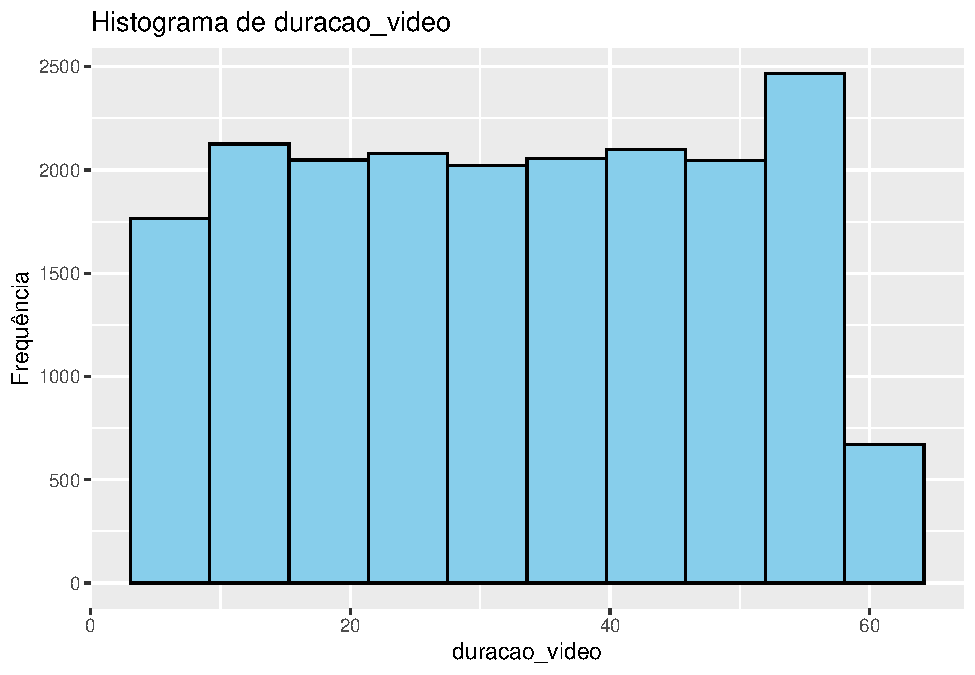
\includegraphics{dados_videos_files/figure-latex/histogramas_variaveis-1.pdf}
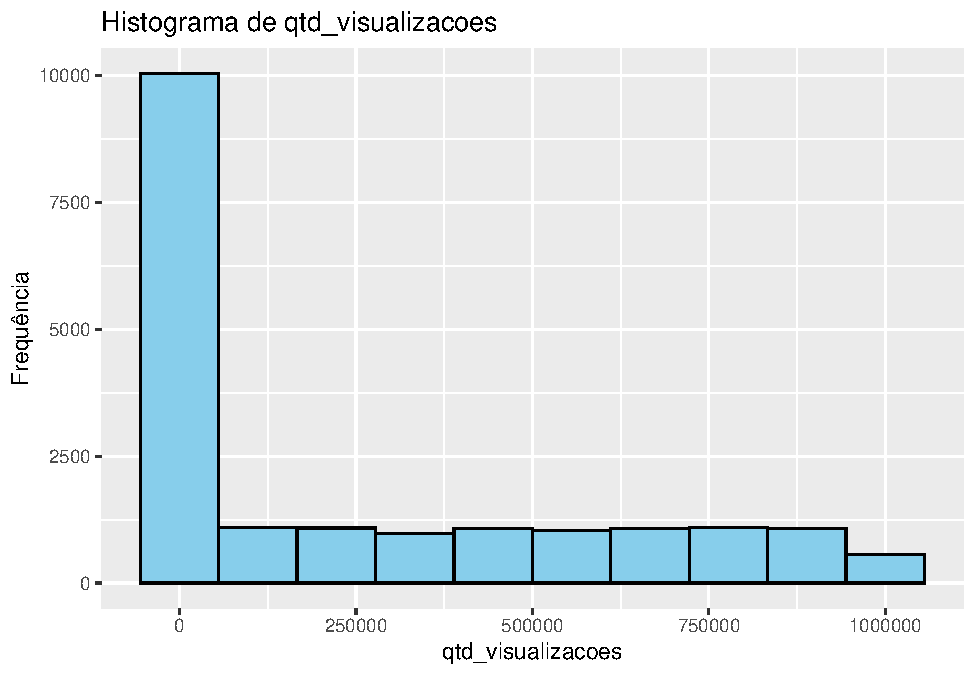
\includegraphics{dados_videos_files/figure-latex/histogramas_variaveis-2.pdf}
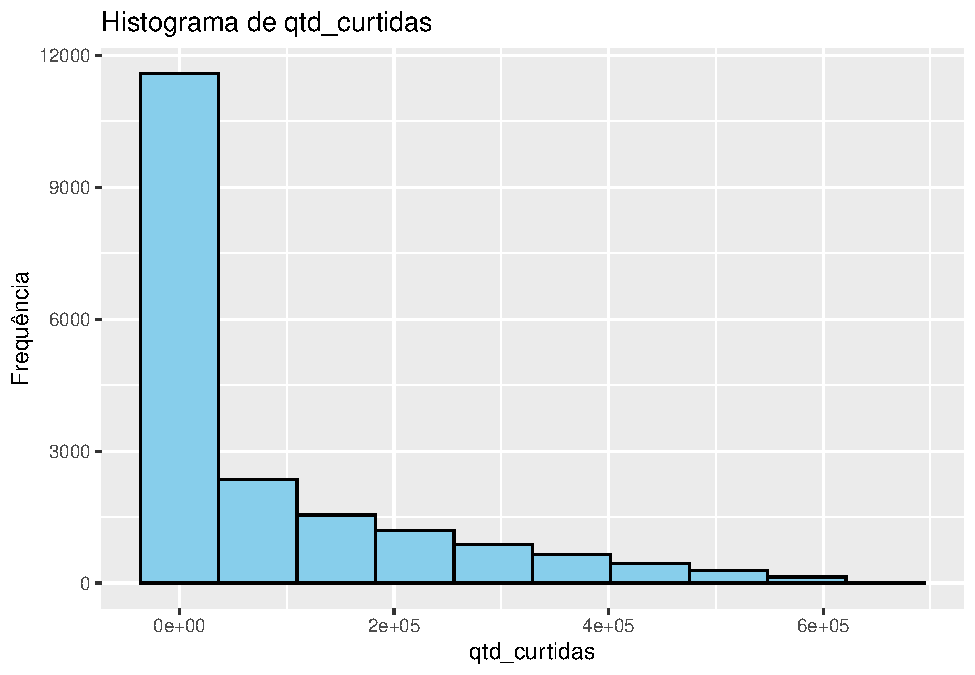
\includegraphics{dados_videos_files/figure-latex/histogramas_variaveis-3.pdf}
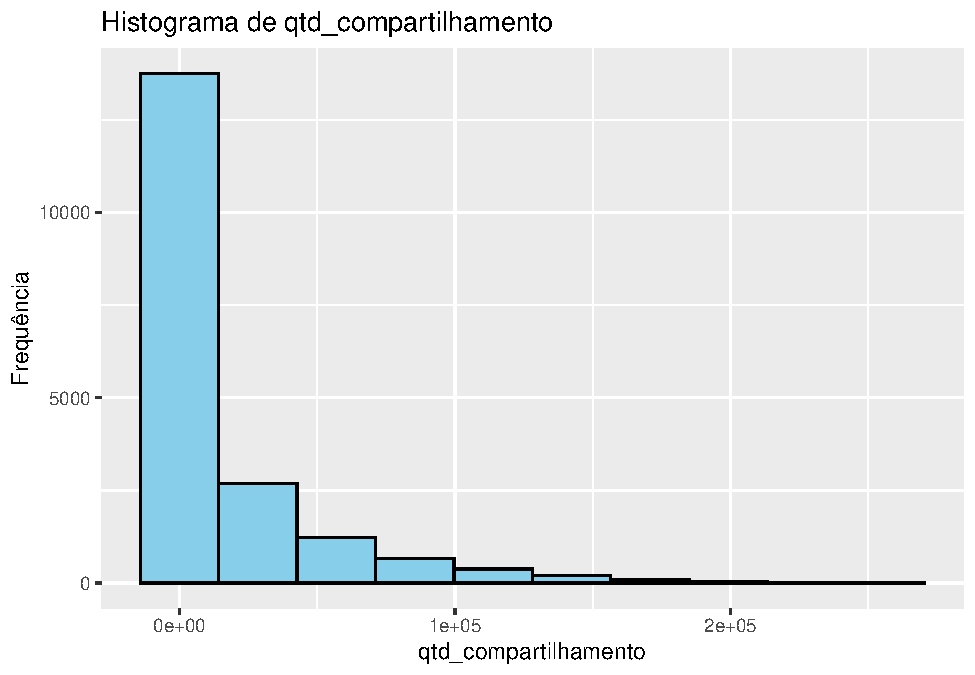
\includegraphics{dados_videos_files/figure-latex/histogramas_variaveis-4.pdf}
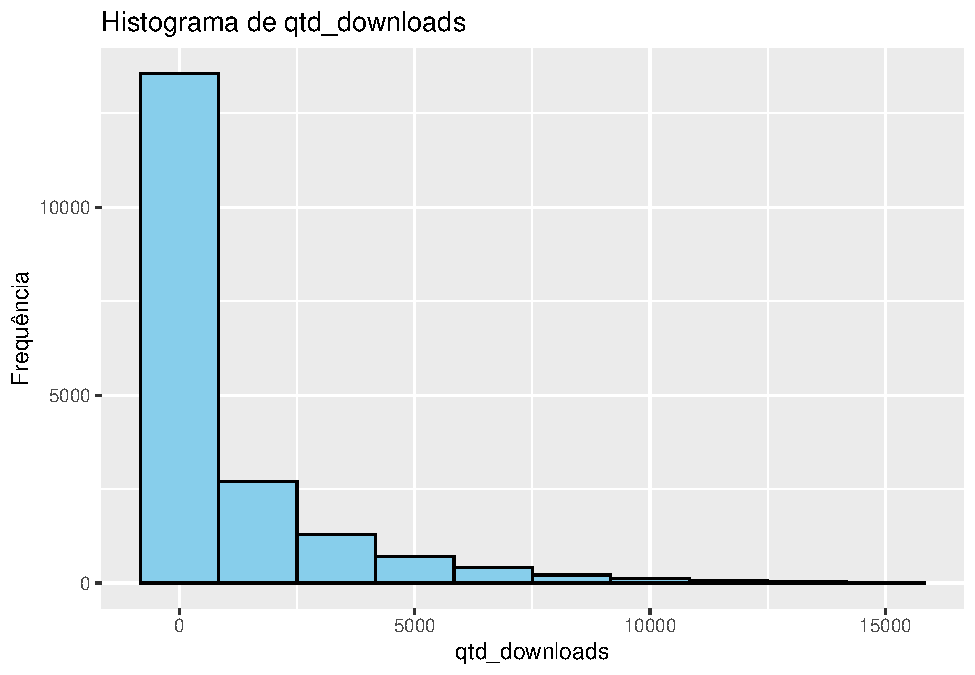
\includegraphics{dados_videos_files/figure-latex/histogramas_variaveis-5.pdf}
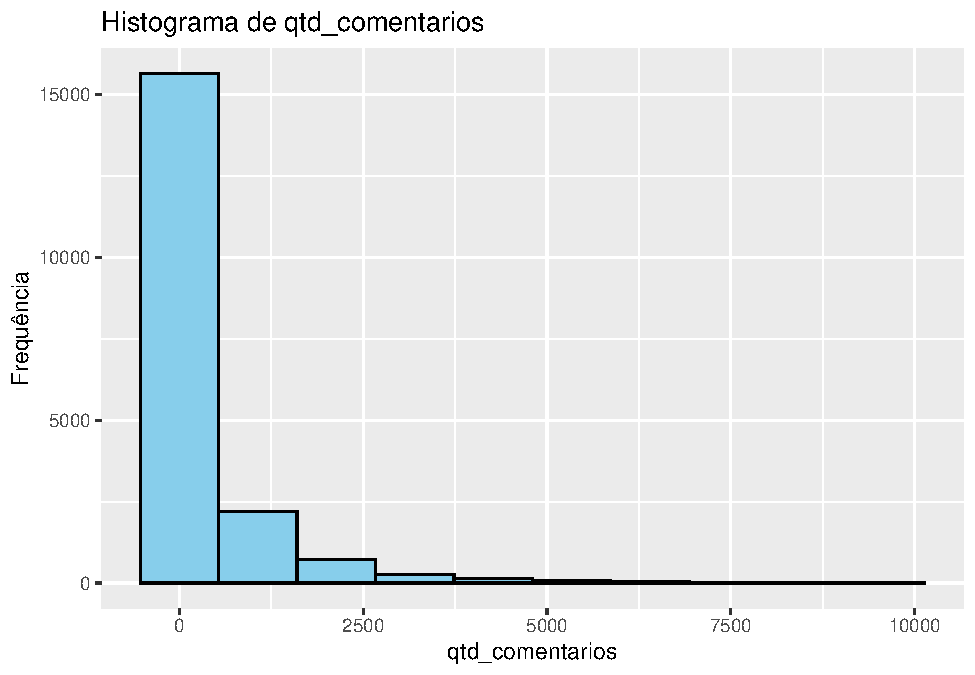
\includegraphics{dados_videos_files/figure-latex/histogramas_variaveis-6.pdf}

\subsection{5C. Q-Q Plot por
Variável}\label{c.-q-q-plot-por-variuxe1vel}

\begin{Shaded}
\begin{Highlighting}[]
\ControlFlowTok{for}\NormalTok{ (var }\ControlFlowTok{in}\NormalTok{ variaveis) \{}
  \FunctionTok{print}\NormalTok{(}
    \FunctionTok{ggqqplot}\NormalTok{(dados\_videos[[var]], }\AttributeTok{title =} \FunctionTok{paste}\NormalTok{(}\StringTok{"Q{-}Q Plot de"}\NormalTok{, var))}
\NormalTok{  )}
\NormalTok{\}}
\end{Highlighting}
\end{Shaded}

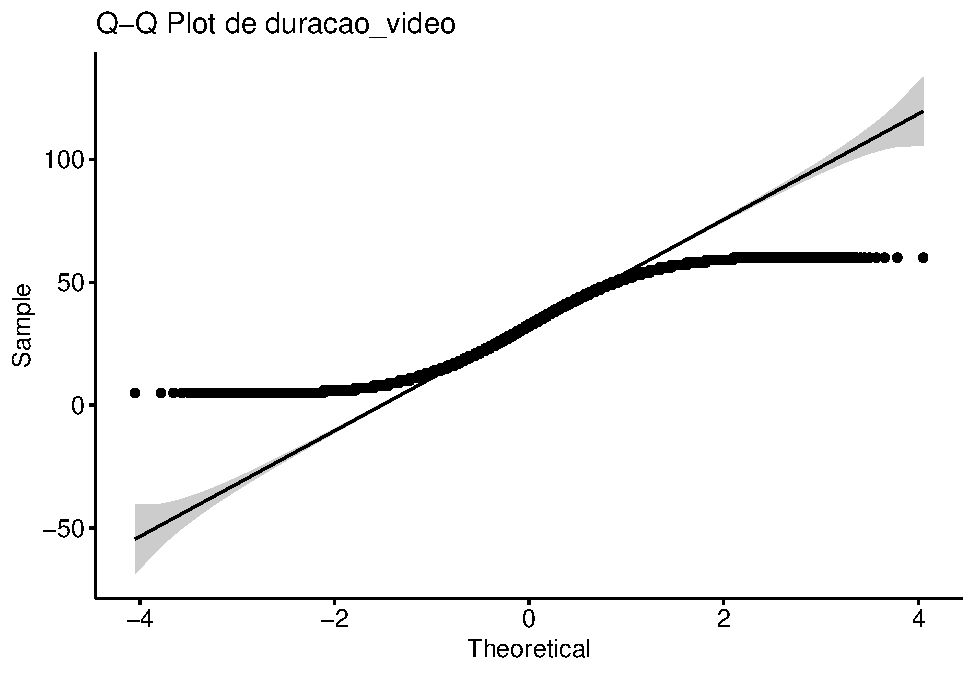
\includegraphics{dados_videos_files/figure-latex/qqplot_variaveis-1.pdf}
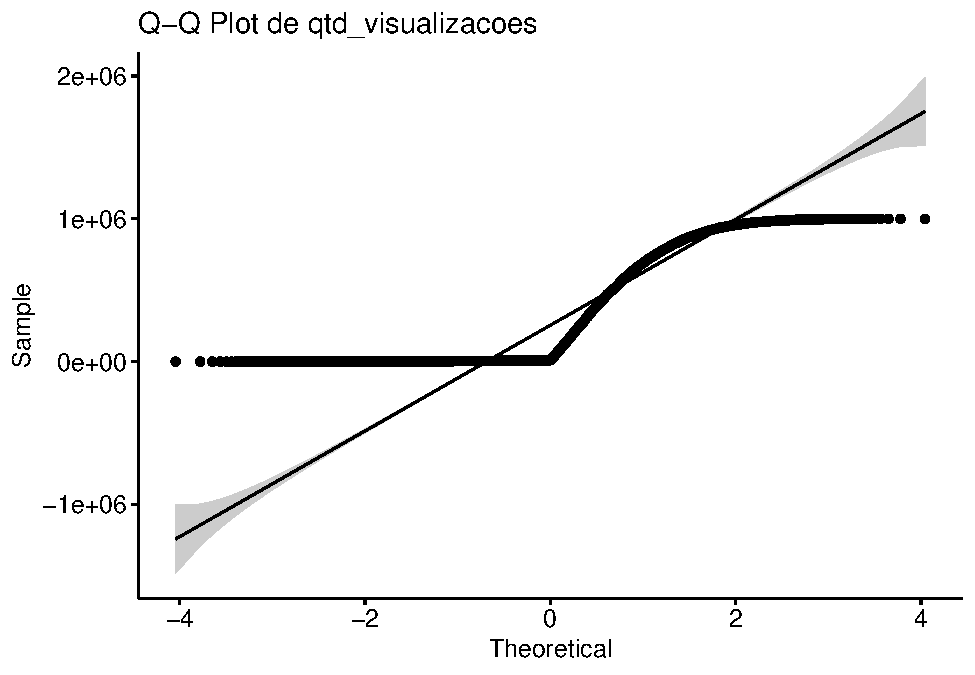
\includegraphics{dados_videos_files/figure-latex/qqplot_variaveis-2.pdf}
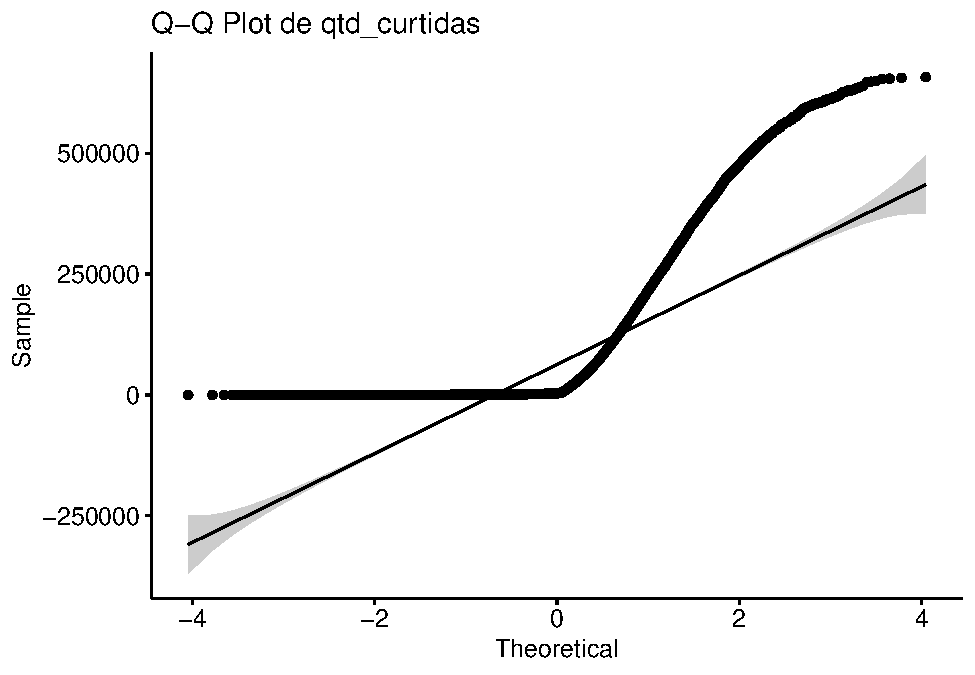
\includegraphics{dados_videos_files/figure-latex/qqplot_variaveis-3.pdf}
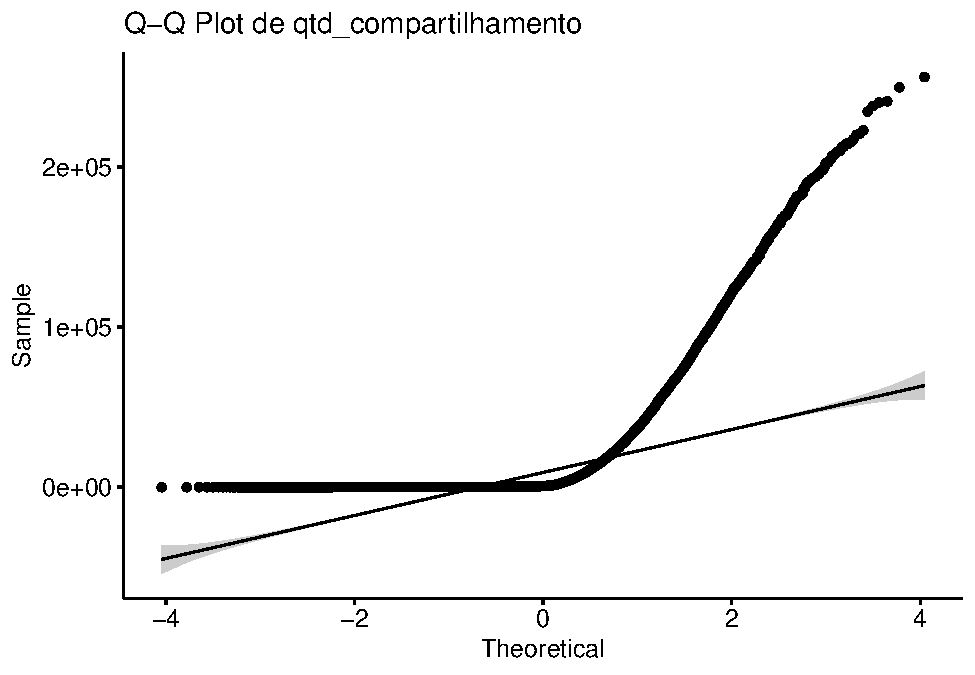
\includegraphics{dados_videos_files/figure-latex/qqplot_variaveis-4.pdf}
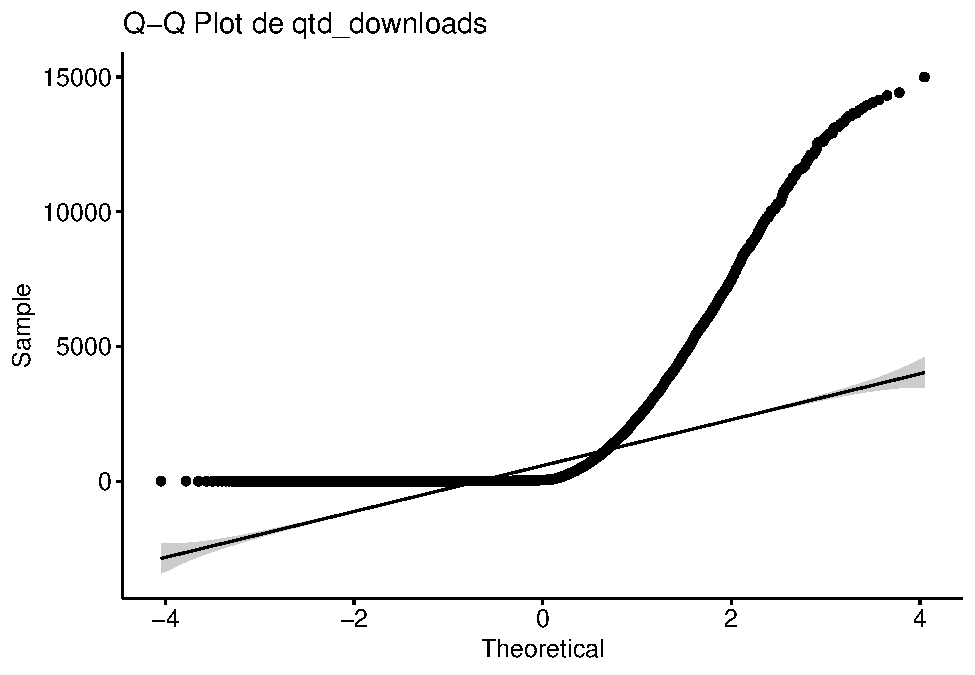
\includegraphics{dados_videos_files/figure-latex/qqplot_variaveis-5.pdf}
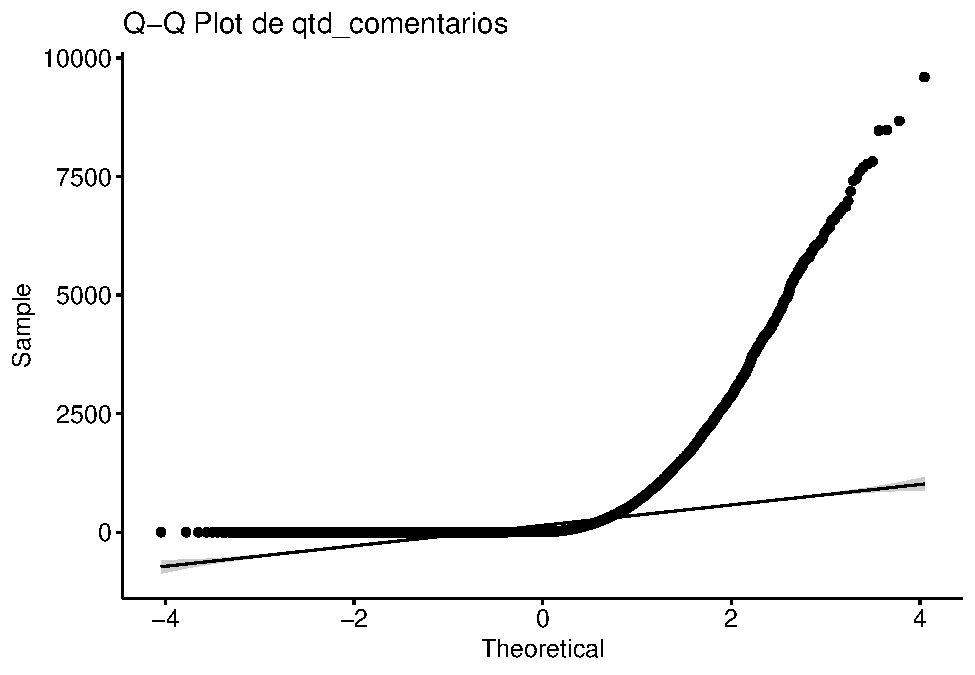
\includegraphics{dados_videos_files/figure-latex/qqplot_variaveis-6.pdf}

\subsection{5D e 5E. Teste de Normalidade
(Shapiro-Wilk)}\label{d-e-5e.-teste-de-normalidade-shapiro-wilk}

\textbf{Desta forma, nenhuma das variáveis numéricas da base de dados
segue uma distribuição normal.}

Segundo o teste de Shapiro-Wilk, rejeita-se a hipótese nula de
normalidade sempre que o p-valor é inferior a 0.05. Neste caso, todos os
p-valores são muito inferiores a esse limite, indicando que os dados não
são normalmente distribuídos.

\begin{Shaded}
\begin{Highlighting}[]
\NormalTok{shapiro\_resultados }\OtherTok{\textless{}{-}} \FunctionTok{sapply}\NormalTok{(dados\_videos[variaveis], }\ControlFlowTok{function}\NormalTok{(x) }\FunctionTok{shapiro.test}\NormalTok{(x)}\SpecialCharTok{$}\NormalTok{p.value)}
\NormalTok{shapiro\_resultados}
\end{Highlighting}
\end{Shaded}

\begin{verbatim}
##        duracao_video    qtd_visualizacoes         qtd_curtidas 
##         5.083467e-35         3.188442e-60         6.863126e-66 
## qtd_compartilhamento        qtd_downloads      qtd_comentarios 
##         2.786075e-71         4.570776e-71         8.155866e-76
\end{verbatim}

\subsection{6. Completude dos Dados}\label{completude-dos-dados}

\subsubsection{Completude: Em pesquisa ao dicionário Oxford, seria
referido a algo como qualidade, estado ou propriedade do que é completo,
perfeito,
acabado.}\label{completude-em-pesquisa-ao-dicionuxe1rio-oxford-seria-referido-a-algo-como-qualidade-estado-ou-propriedade-do-que-uxe9-completo-perfeito-acabado.}

Mas para a visão dos dados, seria algo referente a ter todas as
informações necessárias presentes no conjunto, no caso, ter os dados
inteiros, sem colunas ou linhas vazias, campos nulos e afins. E isso é
totalmente um dos pilares quando falamos em qualidade dos dados, porque
sempre buscamos a confiabilidade, consistência e que sejam dados
totalmente confiáveis. E o impacto na análise exploratória de dados
(EDA) é praticamente o que significa a completude, a busca para que
possamos fazer com que os dados sejam de máxima credibilidade,
assertivos, consistentes e essa ação de tratar os dados, é para
buscarmos a qualidade de completude ao negócio, pesquisa ou afins.

Podemos abordar diversas práticas de governança, metodologias e afins,
mas organizações avançadas sempre estão monitorando a completude de seus
dados, justamente por ser facilmente mensurável e diretamente ligado à
confiança nas análises.

Por isso, a completude de dados não é apenas uma questão técnica --- é
também uma questão de credibilidade. Sem dados completos, a análise
deixa de ser levada em consideração no negócio e passa a ser um
empecilho, já que os dados são extremamente importantes para apoiar
decisões estratégicas, e caso não tenhamos visão clara disso tudo, é
como andar de carro, subindo uma serra cheia de neblina, um perigo
enorme.

\subsection{7. Completude dos Dados}\label{completude-dos-dados-1}

\begin{Shaded}
\begin{Highlighting}[]
\NormalTok{completude }\OtherTok{\textless{}{-}} \FunctionTok{sapply}\NormalTok{(dados\_videos, }\ControlFlowTok{function}\NormalTok{(x) }\FunctionTok{sum}\NormalTok{(}\SpecialCharTok{!}\FunctionTok{is.na}\NormalTok{(x)) }\SpecialCharTok{/} \FunctionTok{length}\NormalTok{(x))}
\NormalTok{completude}
\end{Highlighting}
\end{Shaded}

\begin{verbatim}
##             video_id status_reinvidicacao        duracao_video 
##            1.0000000            0.9854404            1.0000000 
##    transcricao_video   status_verificacao         status_video 
##            0.9854404            1.0000000            1.0000000 
##    qtd_visualizacoes         qtd_curtidas qtd_compartilhamento 
##            0.9854404            0.9854404            0.9854404 
##        qtd_downloads      qtd_comentarios 
##            0.9854404            0.9854404
\end{verbatim}

\subsection{8. Imputação de Dados com
MICE}\label{imputauxe7uxe3o-de-dados-com-mice}

\begin{Shaded}
\begin{Highlighting}[]
\NormalTok{imp }\OtherTok{\textless{}{-}} \FunctionTok{mice}\NormalTok{(dados\_videos, }\AttributeTok{m =} \DecValTok{5}\NormalTok{, }\AttributeTok{method =} \StringTok{"pmm"}\NormalTok{, }\AttributeTok{seed =} \DecValTok{123}\NormalTok{)}
\end{Highlighting}
\end{Shaded}

\begin{verbatim}
## 
##  iter imp variable
##   1   1  qtd_visualizacoes  qtd_curtidas  qtd_compartilhamento  qtd_downloads  qtd_comentarios
##   1   2  qtd_visualizacoes  qtd_curtidas  qtd_compartilhamento  qtd_downloads  qtd_comentarios
##   1   3  qtd_visualizacoes  qtd_curtidas  qtd_compartilhamento  qtd_downloads  qtd_comentarios
##   1   4  qtd_visualizacoes  qtd_curtidas  qtd_compartilhamento  qtd_downloads  qtd_comentarios
##   1   5  qtd_visualizacoes  qtd_curtidas  qtd_compartilhamento  qtd_downloads  qtd_comentarios
##   2   1  qtd_visualizacoes  qtd_curtidas  qtd_compartilhamento  qtd_downloads  qtd_comentarios
##   2   2  qtd_visualizacoes  qtd_curtidas  qtd_compartilhamento  qtd_downloads  qtd_comentarios
##   2   3  qtd_visualizacoes  qtd_curtidas  qtd_compartilhamento  qtd_downloads  qtd_comentarios
##   2   4  qtd_visualizacoes  qtd_curtidas  qtd_compartilhamento  qtd_downloads  qtd_comentarios
##   2   5  qtd_visualizacoes  qtd_curtidas  qtd_compartilhamento  qtd_downloads  qtd_comentarios
##   3   1  qtd_visualizacoes  qtd_curtidas  qtd_compartilhamento  qtd_downloads  qtd_comentarios
##   3   2  qtd_visualizacoes  qtd_curtidas  qtd_compartilhamento  qtd_downloads  qtd_comentarios
##   3   3  qtd_visualizacoes  qtd_curtidas  qtd_compartilhamento  qtd_downloads  qtd_comentarios
##   3   4  qtd_visualizacoes  qtd_curtidas  qtd_compartilhamento  qtd_downloads  qtd_comentarios
##   3   5  qtd_visualizacoes  qtd_curtidas  qtd_compartilhamento  qtd_downloads  qtd_comentarios
##   4   1  qtd_visualizacoes  qtd_curtidas  qtd_compartilhamento  qtd_downloads  qtd_comentarios
##   4   2  qtd_visualizacoes  qtd_curtidas  qtd_compartilhamento  qtd_downloads  qtd_comentarios
##   4   3  qtd_visualizacoes  qtd_curtidas  qtd_compartilhamento  qtd_downloads  qtd_comentarios
##   4   4  qtd_visualizacoes  qtd_curtidas  qtd_compartilhamento  qtd_downloads  qtd_comentarios
##   4   5  qtd_visualizacoes  qtd_curtidas  qtd_compartilhamento  qtd_downloads  qtd_comentarios
##   5   1  qtd_visualizacoes  qtd_curtidas  qtd_compartilhamento  qtd_downloads  qtd_comentarios
##   5   2  qtd_visualizacoes  qtd_curtidas  qtd_compartilhamento  qtd_downloads  qtd_comentarios
##   5   3  qtd_visualizacoes  qtd_curtidas  qtd_compartilhamento  qtd_downloads  qtd_comentarios
##   5   4  qtd_visualizacoes  qtd_curtidas  qtd_compartilhamento  qtd_downloads  qtd_comentarios
##   5   5  qtd_visualizacoes  qtd_curtidas  qtd_compartilhamento  qtd_downloads  qtd_comentarios
\end{verbatim}

\begin{Shaded}
\begin{Highlighting}[]
\NormalTok{dados\_imputados }\OtherTok{\textless{}{-}} \FunctionTok{complete}\NormalTok{(imp, }\DecValTok{1}\NormalTok{)}
\FunctionTok{head}\NormalTok{(dados\_imputados)}
\end{Highlighting}
\end{Shaded}

\begin{verbatim}
##   video_id status_reinvidicacao duracao_video
## 1        1                claim            59
## 2        2                claim            32
## 3        3                claim            31
## 4        4                claim            25
## 5        5                claim            19
## 6        6                claim            35
##                                                                                                                           transcricao_video
## 1                                         someone shared with me that drone deliveries are already happening and will become common by 2025
## 2                               someone shared with me that there are more microorganisms in one teaspoon of soil than people on the planet
## 3 someone shared with me that american industrialist andrew carnegie had a net worth of $475 million usd, worth over $300 billion usd today
## 4       someone shared with me that the metro of st. petersburg, with an average depth of hundred meters, is the deepest metro in the world
## 5          someone shared with me that the number of businesses allowing employees to bring pets to the workplace has grown by 6% worldwide
## 6           someone shared with me that gross domestic product (gdp) is the best financial indicator of a country's overall trade potential
##   status_verificacao status_video qtd_visualizacoes qtd_curtidas
## 1       not verified under review            343296        19425
## 2       not verified       active            140877        77355
## 3       not verified       active            902185        97690
## 4       not verified       active            437506       239954
## 5       not verified       active             56167        34987
## 6       not verified under review            336647       175546
##   qtd_compartilhamento qtd_downloads qtd_comentarios
## 1                  241             1               0
## 2                19034          1161             684
## 3                 2858           833             329
## 4                34812          1234             584
## 5                 4110           547             152
## 6                62303          4293            1857
\end{verbatim}

\begin{Shaded}
\begin{Highlighting}[]
\FunctionTok{colSums}\NormalTok{(}\FunctionTok{is.na}\NormalTok{(dados\_imputados))}
\end{Highlighting}
\end{Shaded}

\begin{verbatim}
##             video_id status_reinvidicacao        duracao_video 
##                    0                   60                    0 
##    transcricao_video   status_verificacao         status_video 
##                   60                    0                    0 
##    qtd_visualizacoes         qtd_curtidas qtd_compartilhamento 
##                    0                    0                    0 
##        qtd_downloads      qtd_comentarios 
##                    0                    0
\end{verbatim}

\subsubsection{Verificando quantidade de ajustes foi realizado pelo
Pacote MICE - modelo
2.}\label{verificando-quantidade-de-ajustes-foi-realizado-pelo-pacote-mice---modelo-2.}

\begin{Shaded}
\begin{Highlighting}[]
\FunctionTok{colSums}\NormalTok{(}\FunctionTok{is.na}\NormalTok{(dados\_imputados))}
\end{Highlighting}
\end{Shaded}

\begin{verbatim}
##             video_id status_reinvidicacao        duracao_video 
##                    0                   60                    0 
##    transcricao_video   status_verificacao         status_video 
##                   60                    0                    0 
##    qtd_visualizacoes         qtd_curtidas qtd_compartilhamento 
##                    0                    0                    0 
##        qtd_downloads      qtd_comentarios 
##                    0                    0
\end{verbatim}

\subsection{9. Dashboard com Shiny}\label{dashboard-com-shiny}

\begin{Shaded}
\begin{Highlighting}[]
\CommentTok{\# Interface do usuário}
\NormalTok{ui }\OtherTok{\textless{}{-}} \FunctionTok{fluidPage}\NormalTok{(}
  \FunctionTok{titlePanel}\NormalTok{(}\StringTok{"Dashboard de Vídeos"}\NormalTok{),}
  \FunctionTok{sidebarLayout}\NormalTok{(}
    \FunctionTok{sidebarPanel}\NormalTok{(}
      \FunctionTok{selectInput}\NormalTok{(}\StringTok{"variavel"}\NormalTok{, }\StringTok{"Escolha a variável:"}\NormalTok{, }
                  \AttributeTok{choices =} \FunctionTok{c}\NormalTok{(}\StringTok{"qtd\_visualizacoes"}\NormalTok{, }\StringTok{"qtd\_curtidas"}\NormalTok{, }
                              \StringTok{"qtd\_compartilhamento"}\NormalTok{, }\StringTok{"qtd\_downloads"}\NormalTok{, }\StringTok{"qtd\_comentarios"}\NormalTok{)),}
      \FunctionTok{colourInput}\NormalTok{(}\StringTok{"cor"}\NormalTok{, }\StringTok{"Cor da linha:"}\NormalTok{, }\AttributeTok{value =} \StringTok{"blue"}\NormalTok{),}
      \FunctionTok{sliderInput}\NormalTok{(}\StringTok{"xlim"}\NormalTok{, }\StringTok{"Limite do eixo X:"}\NormalTok{, }\AttributeTok{min =} \DecValTok{0}\NormalTok{, }\AttributeTok{max =} \DecValTok{100}\NormalTok{, }\AttributeTok{value =} \FunctionTok{c}\NormalTok{(}\DecValTok{0}\NormalTok{, }\DecValTok{100}\NormalTok{)),}
      \FunctionTok{sliderInput}\NormalTok{(}\StringTok{"ylim"}\NormalTok{, }\StringTok{"Limite do eixo Y:"}\NormalTok{, }\AttributeTok{min =} \DecValTok{0}\NormalTok{, }\AttributeTok{max =} \DecValTok{1000000}\NormalTok{, }\AttributeTok{value =} \FunctionTok{c}\NormalTok{(}\DecValTok{0}\NormalTok{, }\DecValTok{500000}\NormalTok{))}
\NormalTok{    ),}
    \FunctionTok{mainPanel}\NormalTok{(}
      \FunctionTok{plotOutput}\NormalTok{(}\StringTok{"grafico"}\NormalTok{)  }\CommentTok{\# Corrigido: nome em minúsculo}
\NormalTok{    )}
\NormalTok{  )}
\NormalTok{)}

\CommentTok{\# Servidor}
\NormalTok{server }\OtherTok{\textless{}{-}} \ControlFlowTok{function}\NormalTok{(input, output) \{}
\NormalTok{  output}\SpecialCharTok{$}\NormalTok{grafico }\OtherTok{\textless{}{-}} \FunctionTok{renderPlot}\NormalTok{(\{}
    \FunctionTok{ggplot}\NormalTok{(dados\_videos, }\FunctionTok{aes\_string}\NormalTok{(}\AttributeTok{x =} \StringTok{"duracao\_video"}\NormalTok{, }\AttributeTok{y =}\NormalTok{ input}\SpecialCharTok{$}\NormalTok{variavel)) }\SpecialCharTok{+}
      \FunctionTok{geom\_line}\NormalTok{(}\AttributeTok{color =}\NormalTok{ input}\SpecialCharTok{$}\NormalTok{cor) }\SpecialCharTok{+}
      \FunctionTok{coord\_cartesian}\NormalTok{(}\AttributeTok{xlim =}\NormalTok{ input}\SpecialCharTok{$}\NormalTok{xlim, }\AttributeTok{ylim =}\NormalTok{ input}\SpecialCharTok{$}\NormalTok{ylim) }\SpecialCharTok{+}
      \FunctionTok{labs}\NormalTok{(}\AttributeTok{title =} \FunctionTok{paste}\NormalTok{(}\StringTok{"Gráfico de Linha para"}\NormalTok{, input}\SpecialCharTok{$}\NormalTok{variavel),}
           \AttributeTok{x =} \StringTok{"Duração do Vídeo"}\NormalTok{, }\AttributeTok{y =}\NormalTok{ input}\SpecialCharTok{$}\NormalTok{variavel)}
\NormalTok{  \})}
\NormalTok{\}}

\CommentTok{\# Rodar o app}
\FunctionTok{shinyApp}\NormalTok{(}\AttributeTok{ui =}\NormalTok{ ui, }\AttributeTok{server =}\NormalTok{ server)}
\end{Highlighting}
\end{Shaded}

Foto do Dashboard com Shiny\\
\strut \\
\includegraphics{images/Captura de tela 2025-04-12 213221.png}

\subsection{Referências}\label{referuxeancias}

\begin{itemize}
\tightlist
\item
  Fonte dos dados: base simulada \texttt{dados\_videos.xlsx}
\item
  Pacotes utilizados: \texttt{ggplot2}, \texttt{summarytools},
  \texttt{GGally}, \texttt{ggpubr}, \texttt{mice}, \texttt{shiny},
  \texttt{colourpicker}
\item
  \#10 Código disponibilizado em:
  \url{https://github.com/VinniciusL/EDA2025}
\item
  Curso: Análise Exploratória de Dados com R
\end{itemize}

\end{document}
